\documentclass{beamer}
\usepackage{amsmath,graphics}
\usepackage{amssymb}

\usetheme{default}
\usepackage{xcolor}

\definecolor{solarizedBase03}{HTML}{002B36}
\definecolor{solarizedBase02}{HTML}{073642}
\definecolor{solarizedBase01}{HTML}{586e75}
\definecolor{solarizedBase00}{HTML}{657b83}
\definecolor{solarizedBase0}{HTML}{839496}
\definecolor{solarizedBase1}{HTML}{93a1a1}
\definecolor{solarizedBase2}{HTML}{EEE8D5}
\definecolor{solarizedBase3}{HTML}{FDF6E3}
\definecolor{solarizedYellow}{HTML}{B58900}
\definecolor{solarizedOrange}{HTML}{CB4B16}
\definecolor{solarizedRed}{HTML}{DC322F}
\definecolor{solarizedMagenta}{HTML}{D33682}
\definecolor{solarizedViolet}{HTML}{6C71C4}
%\definecolor{solarizedBlue}{HTML}{268BD2}
\definecolor{solarizedBlue}{HTML}{134676}
\definecolor{solarizedCyan}{HTML}{2AA198}
\definecolor{solarizedGreen}{HTML}{859900}
\definecolor{myBlue}{HTML}{162DB0}%{261CA4}
\setbeamercolor*{item}{fg=myBlue}
\setbeamercolor{normal text}{fg=solarizedBase03, bg=solarizedBase3}
\setbeamercolor{alerted text}{fg=myBlue}
\setbeamercolor{example text}{fg=myBlue, bg=solarizedBase3}
\setbeamercolor*{frametitle}{fg=solarizedRed}
\setbeamercolor*{title}{fg=solarizedRed}
\setbeamercolor{block title}{fg=myBlue, bg=solarizedBase3}
\setbeameroption{hide notes}
\setbeamertemplate{note page}[plain]
\beamertemplatenavigationsymbolsempty
\usefonttheme{professionalfonts}
\usefonttheme{serif}

\usepackage{fourier}

\def\vec#1{\mathchoice{\mbox{\boldmath$\displaystyle#1$}}
{\mbox{\boldmath$\textstyle#1$}}
{\mbox{\boldmath$\scriptstyle#1$}}
{\mbox{\boldmath$\scriptscriptstyle#1$}}}
\definecolor{OwnGrey}{rgb}{0.560,0.000,0.000} % #999999
\definecolor{OwnBlue}{rgb}{0.121,0.398,0.711} % #1f64b0
\definecolor{red4}{rgb}{0.5,0,0}
\definecolor{blue4}{rgb}{0,0,0.5}
\definecolor{Blue}{rgb}{0,0,0.66}
\definecolor{LightBlue}{rgb}{0.9,0.9,1}
\definecolor{Green}{rgb}{0,0.5,0}
\definecolor{LightGreen}{rgb}{0.9,1,0.9}
\definecolor{Red}{rgb}{0.9,0,0}
\definecolor{LightRed}{rgb}{1,0.9,0.9}
\definecolor{White}{gray}{1}
\definecolor{Black}{gray}{0}
\definecolor{LightGray}{gray}{0.8}
\definecolor{Orange}{rgb}{0.1,0.2,1}
\setbeamerfont{sidebar right}{size=\scriptsize}
\setbeamercolor{sidebar right}{fg=Black}

\renewcommand{\emph}[1]{{\textcolor{solarizedRed}{\itshape #1}}}

\newcommand\cA{\mathcal A}
\newcommand\cB{\mathcal B}
\newcommand\cC{\mathcal C}
\newcommand\cD{\mathcal D}
\newcommand\cE{\mathcal E}
\newcommand\cF{\mathcal F}
\newcommand\cG{\mathcal G}
\newcommand\cH{\mathcal H}
\newcommand\cI{\mathcal I}
\newcommand\cJ{\mathcal J}
\newcommand\cK{\mathcal K}
\newcommand\cL{\mathcal L}
\newcommand\cM{\mathcal M}
\newcommand\cN{\mathcal N}
\newcommand\cO{\mathcal O}
\newcommand\cP{\mathcal P}
\newcommand\cQ{\mathcal Q}
\newcommand\cR{\mathcal R}
\newcommand\cS{\mathcal S}
\newcommand\cT{\mathcal T}
\newcommand\cU{\mathcal U}
\newcommand\cV{\mathcal V}
\newcommand\cW{\mathcal W}
\newcommand\cX{\mathcal X}
\newcommand\cY{\mathcal Y}
\newcommand\cZ{\mathcal Z}

\newcommand\fA{\mathfrak A}
\newcommand\fB{\mathfrak B}
\newcommand\fC{\mathfrak C}
\newcommand\fD{\mathfrak D}
\newcommand\fE{\mathfrak E}
\newcommand\fF{\mathfrak F}
\newcommand\fG{\mathfrak G}
\newcommand\fH{\mathfrak H}
\newcommand\fI{\mathfrak I}
\newcommand\fJ{\mathfrak J}
\newcommand\fK{\mathfrak K}
\newcommand\fL{\mathfrak L}
\newcommand\fM{\mathfrak M}
\newcommand\fN{\mathfrak N}
\newcommand\fO{\mathfrak O}
\newcommand\fP{\mathfrak P}
\newcommand\fQ{\mathfrak Q}
\newcommand\fR{\mathfrak R}
\newcommand\fS{\mathfrak S}
\newcommand\fT{\mathfrak T}
\newcommand\fU{\mathfrak U}
\newcommand\fV{\mathfrak V}
\newcommand\fW{\mathfrak W}
\newcommand\fX{\mathfrak X}
\newcommand\fY{\mathfrak Y}
\newcommand\fZ{\mathfrak Z}

\newcommand\fa{\mathfrak a}
\newcommand\fb{\mathfrak b}
\newcommand\fc{\mathfrak c}
\newcommand\fd{\mathfrak d}
\newcommand\fe{\mathfrak e}
\newcommand\ff{\mathfrak f}
\newcommand\fg{\mathfrak g}
\newcommand\fh{\mathfrak h}
%\newcommand\fi{\mathfrak i}
\newcommand\fj{\mathfrak j}
\newcommand\fk{\mathfrak k}
\newcommand\fl{\mathfrak l}
\newcommand\fm{\mathfrak m}
\newcommand\fn{\mathfrak n}
\newcommand\fo{\mathfrak o}
\newcommand\fp{\mathfrak p}
\newcommand\fq{\mathfrak q}
\newcommand\fr{\mathfrak r}
\newcommand\fs{\mathfrak s}
\newcommand\ft{\mathfrak t}
\newcommand\fu{\mathfrak u}
\newcommand\fv{\mathfrak v}
\newcommand\fw{\mathfrak w}
\newcommand\fx{\mathfrak x}
\newcommand\fy{\mathfrak y}
\newcommand\fz{\mathfrak z}

\newcommand\vA{\vec A}
\newcommand\vB{\vec B}
\newcommand\vC{\vec C}
\newcommand\vD{\vec D}
\newcommand\vE{\vec E}
\newcommand\vF{\vec F}
\newcommand\vG{\vec G}
\newcommand\vH{\vec H}
\newcommand\vI{\vec I}
\newcommand\vJ{\vec J}
\newcommand\vK{\vec K}
\newcommand\vL{\vec L}
\newcommand\vM{\vec M}
\newcommand\vN{\vec N}
\newcommand\vO{\vec O}
\newcommand\vP{\vec P}
\newcommand\vQ{\vec Q}
\newcommand\vR{\vec R}
\newcommand\vS{\vec S}
\newcommand\vT{\vec T}
\newcommand\vU{\vec U}
\newcommand\vV{\vec V}
\newcommand\vW{\vec W}
\newcommand\vX{\vec X}
\newcommand\vY{\vec Y}
\newcommand\vZ{\vec Z}

\newcommand\va{\vec a}
\newcommand\vb{\vec b}
\newcommand\vc{\vec c}
\newcommand\vd{\vec d}
\newcommand\ve{\vec e}
\newcommand\vf{\vec f}
\newcommand\vg{\vec g}
\newcommand\vh{\vec h}
\newcommand\vi{\vec i}
\newcommand\vj{\vec j}
\newcommand\vk{\vec k}
\newcommand\vl{\vec l}
\newcommand\vm{\vec m}
\newcommand\vn{\vec n}
\newcommand\vo{\vec o}
\newcommand\vp{\vec p}
\newcommand\vq{\vec q}
\newcommand\vr{\vec r}
\newcommand\vs{\vec s}
\newcommand\vt{\vec t}
\newcommand\vu{\vec u}
\newcommand\vv{\vec v}
\newcommand\vw{\vec w}
\newcommand\vx{\vec x}
\newcommand\vy{\vec y}
\newcommand\vz{\vec z}

\renewcommand\AA{\mathbb A}
\newcommand\NN{\mathbb N}
\newcommand\ZZ{\mathbb Z}
\newcommand\PP{\mathbb P}
\newcommand\QQ{\mathbb Q}
\newcommand\RR{\mathbb R}
\renewcommand\SS{\mathbb S}
\newcommand\CC{\mathbb C}

\newcommand{\ord}{\mathrm{ord}}
\newcommand{\id}{\mathrm{id}}
\newcommand{\pr}{\mathrm{P}}
\newcommand{\Vol}{\mathrm{vol}}
\newcommand\norm[1]{\left\|{#1}\right\|} 
\newcommand\sign{\mathrm{sign}}
\newcommand{\eps}{\varepsilon}
\newcommand{\abs}[1]{\left|#1\right|}
\newcommand\bc[1]{\left({#1}\right)} 
\newcommand\cbc[1]{\left\{{#1}\right\}} 
\newcommand\bcfr[2]{\bc{\frac{#1}{#2}}} 
\newcommand{\bck}[1]{\left\langle{#1}\right\rangle} 
\newcommand\brk[1]{\left\lbrack{#1}\right\rbrack} 
\newcommand\scal[2]{\bck{{#1},{#2}}} 
\newcommand{\vecone}{\mathbb{1}}
\newcommand{\tensor}{\otimes}
\newcommand{\diag}{\mathrm{diag}}
\newcommand{\ggt}{\mathrm{ggT}}
\newcommand{\kgv}{\mathrm{kgV}}
\newcommand{\trans}{\top}

\newcommand{\Karonski}{Karo\'nski}
\newcommand{\Erdos}{Erd\H{o}s}
\newcommand{\Renyi}{R\'enyi}
\newcommand{\Lovasz}{Lov\'asz}
\newcommand{\Juhasz}{Juh\'asz}
\newcommand{\Bollobas}{Bollob\'as}
\newcommand{\Furedi}{F\"uredi}
\newcommand{\Komlos}{Koml\'os}
\newcommand{\Luczak}{\L uczak}
\newcommand{\Kucera}{Ku\v{c}era}
\newcommand{\Szemeredi}{Szemer\'edi}

\renewcommand{\ae}{\"a}
\renewcommand{\oe}{\"o}
\newcommand{\ue}{\"u}
\newcommand{\Ae}{\"A}
\newcommand{\Oe}{\"O}
\newcommand{\Ue}{\"U}

\newcommand{\im}{\mathrm{im}}
\newcommand{\nul}{\mathrm{nul}}
\newcommand{\rrk}{\mathrm{zrg}}
\newcommand{\crk}{\mathrm{srg}}
\newcommand{\rk}{\mathrm{rg}}
\newcommand{\GL}{\mathrm{GL}}

\newcommand{\mytitle}{Die Dimension}

\title[Linadi]{\mytitle}
\author[Amin Coja-Oghlan]{Amin Coja-Oghlan}
\institute[Frankfurt]{JWGUFFM}
\date{}

\begin{document}

\frame[plain]{\titlepage}

\begin{frame}\frametitle{\mytitle}
	\begin{block}{Definition}
Ein \emph{Untervektorraum} von $\RR^n$ ist eine Menge $E\subseteq\RR^n$, so da\ss\
		\begin{itemize}
			\item $E\neq\emptyset$,
			\item f\ue r alle $u,v\in E$ gilt $u+v\in E$ und
			\item f\ue r alle $u\in E$ und $c\in\RR$ gilt $c\cdot u\in E$.
		\end{itemize}
	\end{block}
	{\itshape Aus der Definition folgt, da\ss\ jeder Untervektorraum den Nullvektor enth\ae lt.}
\end{frame}

\begin{frame}\frametitle{\mytitle}
	\begin{block}{Beispiele}
		\begin{itemize}
			\item $E=\cbc 0$ ist ein Untervektorraum.
			\item $E=\RR^n$ ist ein Untervektorraum.
			\item F\ue r $n=2$ ist
				\begin{align*}
					E=\cbc{\binom{x}{2x}:x\in\RR}
				\end{align*}
				ein Untervektorraum.
			\item Allgemeiner ist f\ue r jedes $v\in\RR^n$ die Menge
				\begin{align*}
					E=\cbc{c\cdot v:c\in\RR}
				\end{align*}
				ein Untervektorraum von $\RR^n$.
		\end{itemize}
	\end{block}
\end{frame}

\begin{frame}\frametitle{\mytitle}
	\begin{block}{Proposition}
		Sei $A$ eine $m\times n$-Matrix.
		\begin{itemize}
			\item $\ker(A)\subseteq\RR^n$ ist ein Untervektorraum.
			\item $\im(A)\subseteq\RR^m$ ist ein Untervektorraum.
		\end{itemize}
	\end{block}
\end{frame}

\begin{frame}\frametitle{\mytitle}
	\begin{block}{Proposition}
		F\ue r jeden Untervektorraum $E\subseteq\RR^n$ existiert eine $n\times n$-Matrix $A$, so da\ss\ $E=\ker(A)$.
	\end{block}
\begin{block}{Proposition}
		F\ue r jeden Untervektorraum $E\subseteq\RR^n$ existiert eine $n\times n$-Matrix $A$, so da\ss\ $E=\im(A)$.
	\end{block}
\end{frame}

\begin{frame}\frametitle{\mytitle}
\begin{block}{Definition}
	Sei $E\subseteq\RR^n$ ein Untervektorraum und sei $A$ eine $n\times n$-Matrix mit $E=\im(A)$.
		Die \emph{Dimension} von $E$ ist definiert als
		\begin{align*}
			\dim(E)&=\rk(A).
		\end{align*}
	\end{block}
	\begin{block}{Anmerkung}
	\begin{itemize}
		\item Die Dimension ist wohldefiniert, d.h.\ je zwei Matrizen $A,A'$ mit $E=\im(A)=\im(A')$ haben denselben Rang.
		\item Es gilt $0\leq\dim(E)\leq n$.
		\item $\dim(E)=0$ genau dann, wenn $E=\cbc0$.
		\item $\dim(E)=n$ genau dann, wenn $E=\RR^n$.
	\end{itemize}	
	\end{block}
\end{frame}

\begin{frame}\frametitle{\mytitle}
\begin{block}{Satz}
	Sei $E\subseteq\RR^n$ ein Untervektorraum und sei $A$ eine $m\times n$-Matrix mit $E=\ker(A)$.
	Dann gilt
	\begin{align*}
		\dim(E)=n-\rk(A).
	\end{align*}
	\end{block}
\end{frame}

\begin{frame}\frametitle{\mytitle}
\begin{block}{Definition}
	Der \emph{Defekt} einer $m\times n$-Matrix $A$ ist definiert als
	\begin{align*}
		\nul(A)=\dim(\ker(A)).
	\end{align*}
	\end{block}
\begin{block}{Dimensionssatz}
	Sei $A$ eine $m\times n$-Matrix.
	Dann gilt
	\begin{align*}
		\nul(A)+\rk(A)=n.
	\end{align*}
\end{block}
\end{frame}

\begin{frame}\frametitle{\mytitle}
\begin{block}{Beispiel}
\begin{itemize}
	\item Die Gerade $E=\cbc{c\cdot\binom{1}2:c\in\RR}\subseteq\RR^2$ ist ein Untervektorraum der Dimension 1, da
		\begin{align*}
			E=\im\begin{pmatrix} 1&0\\2&0 \end{pmatrix}\qquad\mbox{und}\qquad\rk\begin{pmatrix} 1&0\\2&0 \end{pmatrix}=1.
		\end{align*}
	\item F\ue r die Ebene $E=\cbc{\begin{pmatrix}x\\y\\0\end{pmatrix}:x,y\in\RR}\subseteq\RR^3$ gilt
		\begin{align*}
			E&=\ker(A)&\mbox{mit}&&A&=\begin{pmatrix}0&0&0\\0&0&0\\0&0&1\end{pmatrix}.
		\end{align*}
		Aus dem Dimensionssatz folgt $\nul(A)=3-\rk(A)=2$, also $\dim(E)=2$.
\end{itemize}	
\end{block}
\end{frame}

\begin{frame}\frametitle{\mytitle}
	\begin{block}{Definition}
		\begin{itemize}
			\item Seien $v_1,\ldots,v_\ell\in\RR^n$ Vektoren.
			\item Der von $v_1,\ldots,v_\ell$ \emph{erzeugte} oder \emph{aufgespannte Untervektorraum} ist
				\begin{align*}
					\bck{v_1,\ldots,v_\ell}&=\im\bc{v_1\quad\cdots\quad v_\ell}\\
										   &=\cbc{\sum_{i=1}^\ell c_iv_i:c_1,\ldots,c_\ell\in\RR}.
				\end{align*}
		\end{itemize}
	\end{block}
	\begin{block}{Anmerkung}
	\begin{itemize}
	\item Es gilt $\dim\bck{v_1,\ldots,v_\ell}=\rk(v_1\ \cdots\ v_\ell)$.
	\item Die Vektoren $\sum_{i=1}^\ell c_iv_i$ mit $c_1,\ldots,c_\ell\in\RR$ hei\ss en \emph{Linearkombinationen} von $v_1,\ldots,v_\ell$.
	\end{itemize}
		
	\end{block}
\end{frame}

\begin{frame}\frametitle{\mytitle}
	\begin{block}{Definition}
		\begin{itemize}
			\item Seien $v_1,\ldots,v_\ell\in\RR^n$ Vektoren.
			\item Wir nennen $v_1,\ldots,v_\ell$ \emph{linear unabh\ae ngig}, wenn
				\begin{align*}
					\rk(v_1\ \cdots\ v_\ell)&=\ell.
				\end{align*}
			\item Andernfalls sagen wir, $v_1,\ldots,v_\ell$ sind \emph{linear abh\ae ngig}.
		\end{itemize}
	\end{block}
	\begin{block}{Anmerkung}
		Die Vektoren $v_1,\ldots,v_\ell$ sind genau dann linear abh\ae ngig, wenn es $c_1,\ldots,c_\ell\in\RR$ gibt, so da\ss\ $c_i\neq0$ f\ue r ein $i\in\{1,\ldots,\ell\}$ und
		\begin{align*}
			\sum_{i=1}^\ell c_iv_i=0.
		\end{align*}
	\end{block}
\end{frame}

\begin{frame}\frametitle{\mytitle}
	\begin{block}{Beispiel}
		\begin{itemize}
			\item Die Vektoren $\begin{pmatrix}1\\0\\0\end{pmatrix},\begin{pmatrix}0\\1\\0\end{pmatrix},\begin{pmatrix}0\\0\\1\end{pmatrix}$ sind linear unabh\ae ngig, denn
				\begin{align*}
					\rk\begin{pmatrix}1&0&0\\0&1&0\\0&0&1\end{pmatrix}=3.
				\end{align*}
			\item Allgemeiner sind f\ue r jedes $n\in\NN$ die Vektoren
				\begin{align*}
					e^{(i)}_j&=\begin{cases}
						1&\mbox{ falls }i=j\\0&\mbox{ sonst}
					\end{cases}&&(i,j\in\{1,\ldots,n\})
				\end{align*}
				linear unabh\ae ngig.
		\end{itemize}
	\end{block}
\end{frame}

\begin{frame}\frametitle{\mytitle}
	\begin{block}{Beispiel}
		\begin{itemize}
			\item Die Vektoren $\begin{pmatrix} 1\\1\\1 \end{pmatrix}$, $\begin{pmatrix} 2\\2\\2 \end{pmatrix}$ sind linear abh\ae ngig, denn
				\begin{align*}
					\rk\begin{pmatrix}1&2\\1&2\\1&2\end{pmatrix}=1.
				\end{align*}
			\item Wenn einer der Vektoren $v_1,\ldots,v_\ell$ der Nullvektor ist, dann sind $v_1,\ldots,v_\ell$ linear abh\ae ngig.
			\item Ein einzelner Vektor $v_1\neq0$ ist linear unabh\ae ngig.
		\end{itemize}
	\end{block}
\end{frame}

\begin{frame}\frametitle{\mytitle}
	\begin{block}{Definition}
		\begin{itemize}
			\item Sei $E\subseteq\RR^n$ ein Untervektorraum.
			\item Seien $v_1,\ldots,v_\ell\in E$ linear unabh\ae ngig.
			\item Wir nennen $v_1,\ldots,v_\ell$ eine \emph{Basis} von $E$, falls
				\begin{align*}
					E=\bck{v_1,\ldots,v_\ell}.
				\end{align*}
		\end{itemize}
	\end{block}
\end{frame}

\begin{frame}\frametitle{\mytitle}
	\begin{block}{Beispiel}
		\begin{itemize}
			\item Die Vektoren $\begin{pmatrix}1\\0\\0\end{pmatrix},\begin{pmatrix}0\\1\\0\end{pmatrix},\begin{pmatrix}0\\0\\1\end{pmatrix}$ sind eine Basis von $\RR^3$.
			\item Allgemeiner sind f\ue r jedes $n\in\NN$ die Vektoren
				\begin{align*}
					e^{(i)}_j&=\begin{cases}
						1&\mbox{ falls }i=j\\0&\mbox{ sonst}
					\end{cases}&&(i,j\in\{1,\ldots,n\})
				\end{align*}
				eine Basis von $\RR^n$.
		\end{itemize}
	\end{block}
\end{frame}

\begin{frame}\frametitle{\mytitle}
	\begin{block}{Satz}
		\begin{itemize}
			\item Sei $E\subseteq\RR^n$ ein Untervektorraum mit $k=\dim(E)$.
			\item Seien $v_1,\ldots,v_\ell\in E$ linear unabh\ae ngig.
			\item Dann existieren Vektoren $v_{\ell+1},\ldots,v_k\in E$, so da\ss $v_1,\ldots,v_k$ eine Basis von $E$ ist.
		\end{itemize}
	\end{block}
\begin{block}{Korollar}
	Jeder Untervektorraum $E\subseteq\RR^n$ besitzt eine Basis.
	\end{block}
\end{frame}

\begin{frame}\frametitle{\mytitle}
	\begin{block}{Proposition}
		Sei $E$ ein Untervektorraum und sei $v_1,\ldots,v_\ell\in E$ eine Basis.
		Dann gilt $\ell=\dim(E)$ und zu jedem Vektor $u\in E$ existieren eindeutig bestimmte reelle Zahlen $c_1,\ldots,c_\ell$ mit
		\begin{align*}
			u&=\sum_{i=1}^\ell c_iv_i.
		\end{align*}
	\end{block}
\end{frame}

\begin{frame}\frametitle{\mytitle}
	\begin{block}{Beispiel}
	\begin{itemize}
	\item Die Vektoren $\binom10,\binom01$ bilden eine Basis von $\RR^2$; ein Vektor $u\in\RR^2$ kann dargestellt werden in der Form
		\begin{align*}
			u&=u_1\binom10+u_2\binom01.
		\end{align*}
	\end{itemize}
	\end{block}
\end{frame}

\begin{frame}\frametitle{\mytitle}
	\vspace*{-7mm}
	\hfill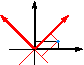
\includegraphics[height=30mm]{pics/basis.pdf}
	\begin{block}{Beispiel}
	\begin{itemize}
	\item Die Vektoren $\binom{\sqrt 2/2}{\sqrt 2/2},\binom{-\sqrt 2/2}{\sqrt 2/2}$ bilden ebenfalls eine Basis von $\RR^2$; ein Vektor $u\in\RR^2$ kann dargestellt werden in der Form
			\begin{align*}
				u&=v_1\cdot\binom{\sqrt 2/2}{\sqrt 2/2}+v_2\binom{-\sqrt 2/2}{\sqrt 2/2}\quad\mbox{mit}&
				v&=\begin{pmatrix} \sqrt 2/2&-\sqrt 2/2\\\sqrt 2/2&\sqrt 2/2 \end{pmatrix}^{-1}u
			\end{align*}
	\item Wir berechnen die inverse Matrix:
		\begin{align*}
			\begin{pmatrix} \sqrt 2/2&-\sqrt 2/2\\\sqrt 2/2&\sqrt 2/2 \end{pmatrix}^{-1}=
			\begin{pmatrix} \sqrt 2/2&\sqrt 2/2\\-\sqrt 2/2&\sqrt 2/2 \end{pmatrix};\quad
\displaystyle v=\begin{pmatrix} \sqrt 2/2&\sqrt 2/2\\-\sqrt 2/2&\sqrt 2/2 \end{pmatrix}u
		\end{align*}
	\end{itemize}
	\end{block}
\end{frame}

\begin{frame}\frametitle{\mytitle}
	\begin{block}{Proposition}
		Sei $v_1,\ldots,v_n$ eine Basis von $\RR^n$ und sei $u\in\RR^n$.
		Dann gilt
		\begin{align*}
			u&=\sum_{i=1}^nc_iv_i&&\mbox{mit}&&c=(v_1\ \cdots\ v_n)^{-1}u.
		\end{align*}
	\end{block}
	\begin{block}{Anmerkung}
		\begin{itemize}
			\item Wir k\oe nnen uns eine Basis von $\RR^n$ also als eine Art Koordinatensystem vorstellen.
			\item Die Koordinaten k\oe nnen durch Matrixinversion bestimmt werden.
		\end{itemize}
	\end{block}
\end{frame}

\begin{frame}\frametitle{\mytitle}
	\begin{block}{Proposition}
		Sei $A$ eine $m\times n$-Matrix vom Rang $k$.
		Dann gibt es eine invertierbare $m\times m$-Matrix $U$ und eine invertierbare $n\times n$-Matrix $V$, so da\ss\
		\begin{align*}
			U^{-1}AV&=B\quad\mbox{mit}\quad B_{ij}=\begin{cases}
				1&\mbox{ falls }i=j\leq k\\
				0&\mbox{ sonst}
			\end{cases}
			\end{align*}
		\end{block}
		\begin{block}{Anmerkung}
			\begin{itemize}
				\item Die Spalten von $U$ und $V$ sind Basen von $\RR^m,\RR^n$.
				\item Bez\ue glich geeigneter Basen besitzt die Matrix $A$ also eine besonders einfache Darstellung.
			\end{itemize}	
		\end{block}
\end{frame}

\begin{frame}\frametitle{\mytitle}
	\begin{block}{Zusammenfassung}
		\begin{itemize}
			\item Jeder Untervektorraum hat eine wohldefinierte Dimension.
			\item Die Dimension ist die Anzahl der Basisvektoren.
			\item Lineare Unabh\ae ngigkeit 
			\item Dimensionssatz
		\end{itemize}
	\end{block}
\end{frame}

\end{document}
